% %% file: template.tex = LaTeX template for article-like report 
%% init: sometime 1993
%% last: Feb  8 2015  Rob Rutten  Deil
%% site: http://www.staff.science.uu.nl/~rutte101/rrweb/rjr-edu/manuals/student-report/

%% First read ``latex-bibtex-simple-manual.txt'' at
%% http://www.staff.science.uu.nl/~rutte101/Report_recipe.html

%% Start your report production by copying this file into your XXXX.tex.
%% Small changes to the header part will make it an A&A or ApJ manuscript.

%%%%%%%%%%%%%%%%%%%%%%%%%%%%%%%%%%%%%%%%%%%%%%%%%%%%%%%%%%%%%%%%%%%%%%%%%%%%
\documentclass{aa}   %% Astronomy & Astrophysics style class
%\documentclass[a4paper,10pt]{report}
\usepackage{graphicx,url,twoopt}
%\usepackage{biblatex}
\usepackage{enumitem}
\usepackage{amsmath}
\usepackage[varg]{txfonts}           %% A&A font choice
%\usepackage{hyperref}                %% for pdflatex
%%\usepackage[breaklinks]{hyperref}  %% for latex+dvips
%%\usepackage{breakurl}              %% for latex+dvips
%\usepackage{pdfcomment}              %% for popup acronym meanings
%\usepackage{acronym}                 %% for popup acronym meanings
\usepackage{calrsfs}
\DeclareMathAlphabet{\pazocal}{OMS}{zplm}{m}{n}

\usepackage{natbib}
% \hypersetup{
%   colorlinks=true,   %% links colored instead of frames
%   urlcolor=blue,     %% external hyperlinks
%   linkcolor=red,     %% internal latex links (eg Fig)
% }

 %\bibpunct{(}{)}{;}{a}{}{,}    %% natbib cite format used by A&A and ApJ
 
 \pagestyle{plain}   %% undo the fancy A&A pagestyle 

%% Add commands to add a note or link to a reference
\makeatletter
\newcommand{\bibnote}[2]{\@namedef{#1note}{#2}}
\newcommand{\biblink}[2]{\@namedef{#1link}{#2}}
\makeatother

%% Commands to make citations ADS clickers and to add such also to refs
%% May 2014: they give error stops ("Illegal parameter number ..."}
%%   for plain latex with TeX Live 2013; the ad-hoc fixes added below let
%%   latex continue instead of stop within these commands.
%%   Please let me know if you know a better fix!
%%   No such problem when using pdflatex.
\makeatletter
 \newcommandtwoopt{\citeads}[3][][]{%
   \nonstopmode%              %% fix to not stop at error message in latex
   \href{http://adsabs.harvard.edu/abs/#3}%
        {\def\hyper@linkstart##1##2{}%
         \let\hyper@linkend\@empty\citealp[#1][#2]{#3}}%   %% Rutten, 2000
   \biblink{#3}{\href{http://adsabs.harvard.edu/abs/#3}{ADS}}%
   \errorstopmode}            %% fix to resume stopping at error messages 
 \newcommandtwoopt{\citepads}[3][][]{%
   \nonstopmode%              %% fix to not stop at error message in latex
   \href{http://adsabs.harvard.edu/abs/#3}%
        {\def\hyper@linkstart##1##2{}%
         \let\hyper@linkend\@empty\citep[#1][#2]{#3}}%     %% (Rutten 2000)
   \biblink{#3}{\href{http://adsabs.harvard.edu/abs/#3}{ADS}}%
   \errorstopmode}            %% fix to resume stopping at error messages
 \newcommandtwoopt{\citetads}[3][][]{%
   \nonstopmode%              %% fix to not stop at error message in latex
   \href{http://adsabs.harvard.edu/abs/#3}%
        {\def\hyper@linkstart##1##2{}%
         \let\hyper@linkend\@empty\citet[#1][#2]{#3}}%     %% Rutten (2000)
   \biblink{#3}{\href{http://adsabs.harvard.edu/abs/#3}{ADS}}%
   \errorstopmode}            %% fix to resume stopping at error messages 
 \newcommandtwoopt{\citeyearads}[3][][]{%
   \nonstopmode%              %% fix to not stop at error message in latex
   \href{http://adsabs.harvard.edu/abs/#3}%
        {\def\hyper@linkstart##1##2{}%
         \let\hyper@linkend\@empty\citeyear[#1][#2]{#3}}%  %% 2000
   \biblink{#3}{\href{http://adsabs.harvard.edu/abs/#3}{ADS}}%
   \errorstopmode}            %% fix to resume stopping at error messages 
\makeatother

%%%%%%%%%%%%%%%%%%%%%%%%%%%%%%%%%%%%%%%%%%%%%%%%%%%%%%%%%%%%%%%%%%%%%%%%%%%%
\begin{document}  

%% simple header.  Change into A&A or ApJ commands for those journals

\twocolumn[{%
\vspace*{4ex}

\begin{center}
  {\Large \bf The recombination history of the universe}\\[4ex]
  {\large \bf Andreas Ellewsen$^1$}\\[4ex]
  \begin{minipage}[t]{15cm}
        $^1$ Institute of Theoretical Astrophysics, University of Oslo, P.O. Box 1029 Blindern, N-0315 Oslo, Norway\\
             
        
    {\bf Abstract.} I compute the electron fraction, electron density, optical depth and visibility function for times around and during recombination. 
    
  \vspace*{2ex}
  \end{minipage}
\end{center}
}]

%%%%%%%%%%%%%%%%%%%%%%%%%%%%%%%%%%%%%%%%%%%%%%%%%%%%%%%%%%%%%%%%%%%%%%%%%%%%
\section{Introduction}\label{sec:introduction}
%%%%%%%%%%%%%%%%%%%%%%%%%%%%%%%%%%%%%%%%%%%%%%%%%%%%%%%%%%%%%%%%%%%%%%%%%%%%
In this project I will follow the algorithm presented in Callin (2005)[1] for simulating the cosmic microwave background.  
This is part two of four for this project.

In the first part I set up the background cosmology of the universe. 
In this part the goal is to compute the optical depth $\tau$ as a function of $x$, where $x$ is the logarithm of the scale factor $a$. And the visibility function $g$, and its scaled version $\tilde{g} = g/\pazocal{H}$. We also want the first and second derivatives of both of these functions with respect to $x$.

As in the first part of the project I will continue building on the skeleton code provided.

%%%%%%%%%%%%%%%%%%%%%%%%%%%%%%%%%%%%%%%%%%%%%%%%%%%%%%%%%%%%%%%%%%%%%%%%%%%%
\section{Equations}\label{sec:Equations}
%%%%%%%%%%%%%%%%%%%%%%%%%%%%%%%%%%%%%%%%%%%%%%%%%%%%%%%%%%%%%%%%%%%%%%%%%%%%
The optical depth is defined
\begin{equation}\label{tau}
 \tau(\eta) = \int_\eta^{\eta_0}n_e\sigma_T ad\eta'.
\end{equation}
This is the probability for a photon to scatter between some previous time $\eta$ and today $\eta_0$. This way, if one at time $\eta$ had a beam of photons with intensity $I_0$ one would today at time $\eta_0$ have a beam with intensity $I = I_0exp(-\tau(\eta))$.
Looking at equation \ref{tau}, $n_e$ is the electron density, $\sigma_T$ the Thompson cross-section, and $a$ the scale factor.

Equation \ref{tau} can be rewritten on differential form as
\begin{equation}\label{tau2}
 \frac{d\tau}{d\eta}  = \dot{\tau}= - n_e\sigma_T a.
\end{equation}
Or since we generally use $x$ instead of $\eta$, as
\begin{equation}
 \frac{d\tau}{dx} = \tau' = -\frac{n_e\sigma_T a}{\pazocal{H}}.
\end{equation}
The Thompson cross section is
\begin{equation}
 \sigma_T =  \frac{8\pi\alpha^2}{3m_e^2} = 6.652462\times10^{-29} \textmd{m}^2.
\end{equation}


The only unknown quantity left in equation \ref{tau2} is $n_e$. 
Before finding a way to compute this quantity we define the visibility function as
\begin{equation}
 g(\eta) = -\dot{\tau}e^{-\tau(\eta)} = \pazocal{H}\tau'e^{-\tau(x)} = g(x)
\end{equation}
\begin{equation}
 \tilde{g}(x) \equiv -\tau'e^{-\tau}=\frac{g(x)}{\pazocal{H}(x)}. 
\end{equation}
This visibility function is normalized as
\begin{equation}
 \int_0^{\eta_0} g(\eta)d\eta = \int_{-\infty}^0 \tilde{g}(x)dx = 1,
\end{equation}
and thus it can be interpreted as a probability distribution. The visibility function then gives the probability that a CMB photon was last scattered at conformal time $\eta$.

From this we see that if we want to find the visibility function $g$, we will need the optical depth $\tau$ and its derivative, and to find that we need the electron density $n_e$.

To find this we will make some assumptions.
We define 
\begin{equation}
 X_e \equiv \frac{n_e}{n_H} = \frac{n_e}{n_b}.
\end{equation}
Note here that we assume that the number density of baryons is equal to the number density of hydrogen. And thus we have ignored all elements above hydrogen. We also ignore the small difference in mass between neutral hydrogen and free protons. Thus we have
\begin{equation}
 n_H = n_b \simeq \frac{\rho_b}{m_H} = \frac{\Omega_b \rho_c}{m_H a^3}
\end{equation}

The only thing left to find now is $X_e$. There are two equations to choose from when calculating this.
One is the Saha equation, which is valid for $X_e \approx 1$. And the other is Peeble's equation which is valid for all values of $X_e$. 

Saha's equation is
\begin{equation}
 \frac{X_e^2}{1-X_e} = \frac{1}{n_b}\bigg(\frac{m_e k_b T_b}{2\pi \hbar^2}\bigg)^{3/2}e^{-\epsilon_0/k_b T_b},
\end{equation}
where $m_e$ is the electron mass, $k_b$ the Boltzmann constant, $T_b$ the baryon temperature, $\hbar$ the reduced Planck constant, and $\epsilon_0$ the ionization energy of hydrogen. This is a regular quadratic equation which can be solved using the regular method.

Peeble's equation is 
\begin{equation}
\frac{dX_e}{dx} = \frac{C_r(T_b)}{H} \left[\beta(T_b)(1-X_e) - n_H
  \alpha^{(2)}(T_b)X_e^2\right],
\end{equation}
where
\begin{align}
C_r(T_b) &= \frac{\Lambda_{2s\rightarrow1s} +	
  \Lambda_{\alpha}}{\Lambda_{2s\rightarrow1s} + \Lambda_{\alpha} +
  \beta^{(2)}(T_b)}, \\  
\Lambda_{2s\rightarrow1s} &= 8.227 \textrm{s}^{-1}\\
\Lambda_{\alpha} &= H\frac{(3\epsilon_0 c/\hbar)^3}{(8\pi)^2 n_{1s}}\\
n_{1s} &= (1-X_e)n_H \\
\beta^{(2)}(T_b) &= \beta(T_b) e^{3\epsilon_0/4k_b T_b} \\
\beta(T_b) &= \alpha^{(2)}(T_b) \left(\frac{m_e k_b T_b}{2\pi\hbar^2}
\right)^{3/2} e^{-\epsilon_0/k_b T_b} \\
\alpha^{(2)}(T_b) &= \frac{64\pi}{\sqrt{27\pi}}
\frac{\hbar^2 \alpha^2}{c m_e^2}\sqrt{\frac{\epsilon_0}{k_b T_b}}\phi_2(T_b)\\
\phi_2(T_b) &= 0.448\ln(\epsilon_0/k_B T_b).
\end{align}
Here $\alpha$ is the fine structure constant.

At early times $X_e$ should be very close to 1, so we will start with Saha's equation. We define the point where we switch from Saha to Peeble's equation at $X_e = 0.99$. 

With this it should be possible to calculate the electron density, optical depth, and the visibility function.
How this is done is explained in the next section.

%%%%%%%%%%%%%%%%%%%%%%%%%%%%%%%%%%%%%%%%%%%%%%%%%%%%%%%%%%%%%%%%%%%%%%%%%%%%
\section{Implementation}\label{sec:Imp}
%%%%%%%%%%%%%%%%%%%%%%%%%%%%%%%%%%%%%%%%%%%%%%%%%%%%%%%%%%%%%%%%%%%%%%%%%%%%
As in part one of the project we will continue using Fortran90.
We will also be using most of the variables we defined in that part again.
The only thing I want to change is the length of my $x$ array. 
Since the evolution of the optical depth should change fairly little except for around recombination, I set it up with three intervals with different step lengths. The first part goes from $x = -10.5$ to the x value corresponding to redshift $z= 1630.4$ with 300 points. The next goes from the end of the first to $z = 614.2$ with 300 points. And the last one goes from there until today at $z = 0$ with 300 points. This ensures that we have a much better resolution around recombination than the rest.

The next step is to calculate the electron density. The first part of this is easy. One writes in the equations and solves the Saha equation with simple algebra. When the switch to Peebles occurs we make use of the ODE solver used in part one of the project. The only change in the implementation is that the guess one does of the appropriate step length is set to one hundredth of the length between two points in the part of $x$ with the smallest resolution. 

With that done we now have $X_e$.
We then use $X_e$ to calculate the electron density $n_e$.

Since we want to be able to find $n_e$ at arbitrary values of $x$ we spline this function. (I actually spline the logarithm of $n_e$ and then exponentiate the answer since $n_e$ varies over so many orders of magnitude.)

Then we use $n_e$ to find $\tau^\prime$, and use the same procedure for the ODE solver to give us $\tau(x)$. Next we spline this function which gives us $\tau^{\prime\prime}$. This makes it possible to write a function which uses the spline to find $\tau(x)$ at arbitrary $x$ values inside the $x$ grid we have used. 

The library which was included with the skeleton code also includes a function that can find $\tau^\prime$ at arbitrary values inside our grid using $\tau$, and $\tau^{\prime\prime}$.

These functions are used to make figure \ref{tau} in section \ref{sec:results}.

Since we now have functions to find $\tau$,$\tau^\prime$, and $\tau^{\prime\prime}$ at any value inside our grid we use them to compute the visibility function. Note that the function I actually implement is not $g$ itself, but rather $\tilde{g}$ as described in section \ref{sec:Equations}.

I use the exact same procedure as I did for $\tau$ to make functions for $\tilde{g}$, $\tilde{g}^\prime$, and $\tilde{g}^{\prime\prime}$.

With this, we have now found $X_e$ and $n_e$, as well as  $\tau$, $g$, and their derivatives. See the next section for figures of these functions.
%%%%%%%%%%%%%%%%%%%%%%%%%%%%%%%%%%%%%%%%%%%%%%%%%%%%%%%%%%%%%%%%%%%%%%%%%%%%
\section{Results}\label{sec:results}
%%%%%%%%%%%%%%%%%%%%%%%%%%%%%%%%%%%%%%%%%%%%%%%%%%%%%%%%%%%%%%%%%%%%%%%%%%%%

The first figure to look at is the one for $X_e$. The observant reader may notice that this plot does not include the whole range of z values which one would assume considering the $x$ range we chose earlier. This is because the electron fraction remains constant at 1 for the entire range until recombination starts around redshift $z = 1600$. As expected once we reach recombination $X_e$ starts dropping quickly. In fact it drops 3 orders of magnitude in the time $z$ goes from $z \approx 1400$ to $z \approx 700$.

  \begin{figure}[ht]
   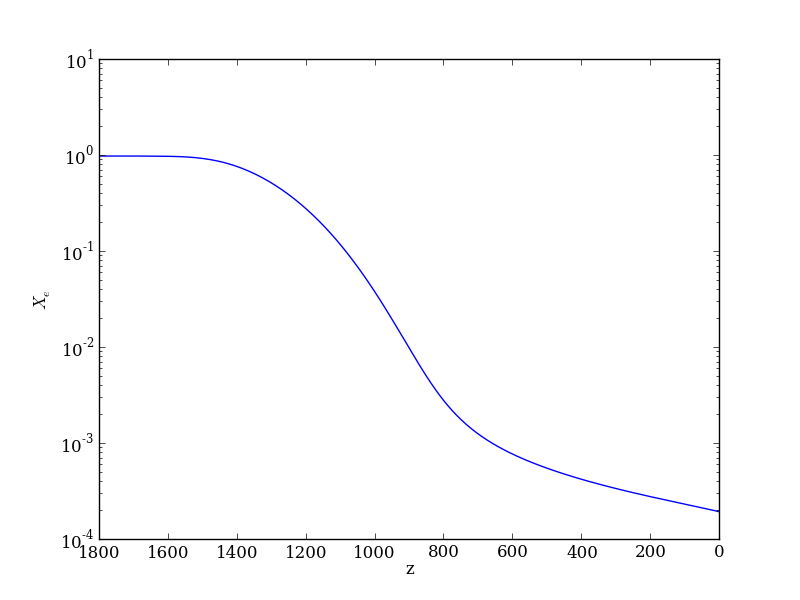
\includegraphics[width=.49\textwidth]{X_e.png}
   \caption{The electron fraction drops quickly during recombination. This would indicate that the optical depth should decrease drastically during the same period. We note that the electron density keeps declining until today. However this has nowhere near the same impact since the universe has already become transparent at that point.}
   \label{fig:X_e}
  \end{figure}

As we expected after looking at the electron fraction there is a steep decline in the optical depth during recombination.
The critical part of this decline is that the optical depth is reduced to levels far lower than 1. This means that the radiation that is sent out is scattered very little before reaching us.


  \begin{figure}[ht]
   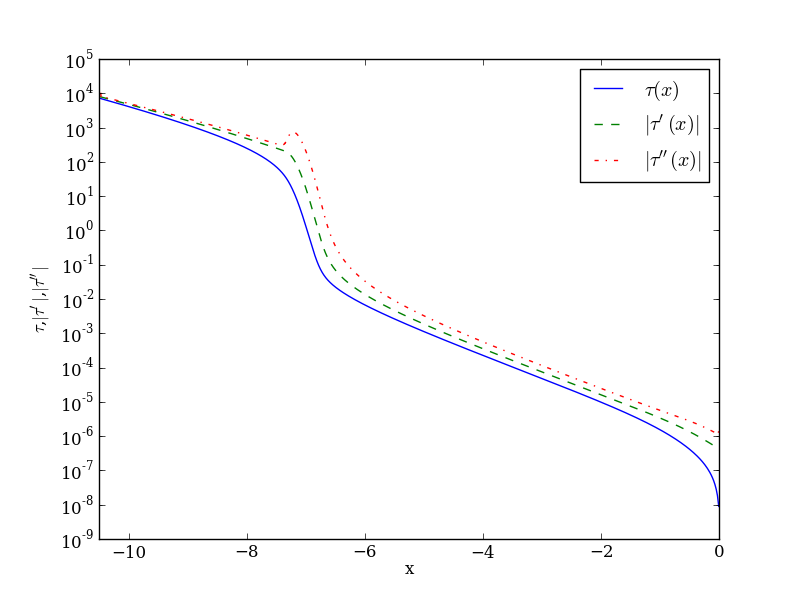
\includegraphics[width=.49\textwidth]{tau.png}
   \caption{The optical depth declines as expected and falls far below 1 causing the universe to become optically thin. This makes it possible for photons to travel freely through the universe, reaching us today without having been scattered again after their initially scattering during recombination.}
   \label{fig:tau}
  \end{figure}
 
Since the photons almost stop getting scattered after recombination one would expect a large peak in the visibility function during this time. (Since the visibility function describes the probability of last begin scattered at some time.) This is exactly what we see in the figure of the visibility function. We get a large peak between redshift $z=-7.2$ and $z=-6.7$. Because of this narrow range this is usually referred to as the last scattering surface.
 
   \begin{figure}[ht]
   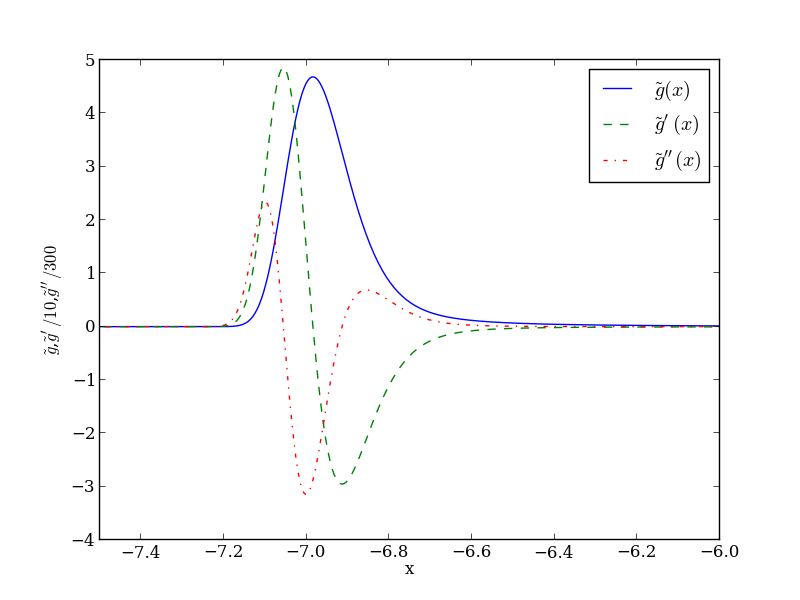
\includegraphics[width=.49\textwidth]{g.png}
   \caption{The figure confirms my expectations from the optical depth, meaning that we get a distinct peak in the visibility function around recombination.}
  \label{fig:g}
  \end{figure}

  
% \begin{table}
%  \begin{tabular}{|c|c|c|}
%   \hline
%   &Analytical &Numerical \\
%   \hline
%   $<E>$ &-1.996 & -1.996\\
%   \hline
%   $<|M|>$& 0.999& 0.999\\
%   \hline
%   $C_V$ & 0.032& 0.032\\
%   \hline
%   $\chi$ & 0.004& 0.004\\
%   \hline
%  \end{tabular}
% \caption{}
% \label{tab1}
% \end{table}

%%%%%%%%%%%%%%%%%%%%%%%%%%%%%%%%%%%%%%%%%%%%%%%%%%%%%%%%%%%%%%%%%%%%%%%%%%%%
\section{Conclusions} \label{sec:conclusions}
%%%%%%%%%%%%%%%%%%%%%%%%%%%%%%%%%%%%%%%%%%%%%%%%%%%%%%%%%%%%%%%%%%%%%%%%%%%%
In this project I have found the electron fraction for time before, during, and after recombination.
This was used to find the optical depth at the same times, which was then used to find the visibility function.
We saw that the electron density declined steeply during recombination, causing the optical depth to pass from values much larger than 1 to values much lower than 1. 
From this one can say that the universe was opaque before, and very nearly transparent for times later than recombination.
This resulted in a sharp peek in the visibility function at this time. Since the visibility function works as a probability function of when a photon was last scattered, this sharp peak indicates that the majority of the photons that existed were scattered in this time period. Because of this this is referred to as the last scattering surface. 
%%%%%%%%%%%%%%%%%%%%%%%%%%%%%%%%%%%%%%%%%%%%%%%%%%%%%%%%%%%%%%%%%%%%%%%%%%%%
\section{References}
%%%%%%%%%%%%%%%%%%%%%%%%%%%%%%%%%%%%%%%%%%%%%%%%%%%%%%%%%%%%%%%%%%%%%%%%%%%%
\begin{enumerate}[label= {[}\arabic*{]} ]
 \item P. Callin, astro-ph/0606683
\end{enumerate}



%\bibliographystyle{aa-note} %% aa.bst but adding links and notes to references
%\raggedright              %% only for adsaa with dvips, not for pdflatex
%\bibliographystyle{unsrt}
%\bibliography{bibliography}{}       %% XXX.bib = your Bibtex entries copied from ADS

\onecolumn 
%%%%%%%%%%%%%%%%%%%%%%%%%%%%%%%%%%%%%%%%%%%%%%%%%%%%%%%%%%%%%%%%%%%%%%%%%%%%
\section{Source code}\label{sec:files}
%%%%%%%%%%%%%%%%%%%%%%%%%%%%%%%%%%%%%%%%%%%%%%%%%%%%%%%%%%%%%%%%%%%%%%%%%%%%
The source code for the rec\_mod file is included for inspection. Note that the code makes use of several different files, one with various parameters, as well as the ODE solver, and the spline. The time\_mod file from part one of the project is obviously used as well.

\begin{verbatim}
module rec_mod
    use healpix_types
    use params
    use time_mod
    use ode_solver
    use spline_1D_mod
    implicit none

    integer(i4b)                          :: n                             !Number of grid points
    real(dp), allocatable, dimension(:)   :: x_rec,a_rec,z_rec             !Grid
    real(dp), allocatable, dimension(:)   :: tau, dtau, ddtau              !Splined tau and derivatives
    real(dp), allocatable, dimension(:)   :: d4tau
    real(dp), allocatable, dimension(:)   :: n_e, n_e2,logn_e,logn_e2      !Splined (log of) n_e
    real(dp), allocatable, dimension(:)   :: g,dg,ddg,d4g                  !Splined visibility function
    real(dp), allocatable, dimension(:)   :: g_test,dg_test,ddg_test       !Splined visibility function
    real(dp), allocatable, dimension(:)   :: H_rec,X_e                     !Variables for H and X_e
    real(dp), allocatable, dimension(:)   :: x_test,n_etest,z_test,a_test  !Used for testing the splines
    real(dp), allocatable, dimension(:)   :: tau_test,dtau_test,ddtau_test !Used for testing the splines
    real(dp)                              :: x_0
    real(dp)                              :: x_test_start
    real(dp)                              :: x_test_end
    integer(i4b),private :: i
contains

  subroutine initialize_rec_mod
    implicit none
    
    integer(i4b) :: n1,n2,n3
    real(dp)     :: saha_limit, y, T_b, n_b, dydx, xmin, xmax, dx, f, n_e0, X_e0, &
		    X_econst, phi2,alpha2,beta,beta2,n1s,lambda_alpha,C_r
    real(dp)     :: eps,hmin,yp1,ypn,h1,h2,h3
    real(dp)     :: z_start_rec, z_end_rec, z_0, x_before_rec,x_start_rec, x_end_rec
    logical(lgt) :: use_saha


    x_test_start = -10.0d0
    x_test_end   = -1.0d0
    saha_limit   = 0.99d0       ! Switch from Saha to Peebles when X_e < 0.99

    !ODE int variables
    eps  = 1.d-10
    hmin = 0.d0
    yp1  = 1.d30
    ypn  = 1.d30

    !Grid sizes 
    n1          = 300                       ! Number of grid points during recombination
    n2          = 200                       ! Number of grid points after recombination
    n3          = 300
    n           = n1 + n2 +n3               ! Total number of grid points
    z_start_rec = 1630.4d0                  ! Redshift of start of recombination
    z_end_rec   = 614.2d0                   ! Redshift of end of recombination
    z_0         = 0.d0                      ! Redshift today

    x_before_rec= -10.5d0                   ! x at start of array
    x_start_rec = -log(1.d0 + z_start_rec)  ! x of start of recombination
    x_end_rec   = -log(1.d0 + z_end_rec)    ! x of end of recombination

    !Allocate all the arrays which will be used
    allocate(x_rec(n))
    allocate(a_rec(n))
    allocate(z_rec(n))
    allocate(H_rec(n))
    allocate(X_e(n))
    allocate(tau(n))
    allocate(dtau(n))
    allocate(ddtau(n))
    allocate(d4tau(n))
    allocate(n_e(n))
    allocate(n_e2(n))
    allocate(logn_e(n))
    allocate(logn_e2(n))
    allocate(g(n))
    allocate(dg(n))
    allocate(ddg(n))
    allocate(d4g(n))
    allocate(x_test(n))
    allocate(z_test(n))
    allocate(a_test(n))
    allocate(n_etest(n))
    allocate(tau_test(n))
    allocate(dtau_test(n))
    allocate(ddtau_test(n))
    allocate(g_test(n))
    allocate(dg_test(n))
    allocate(ddg_test(n))

    !fill test 
    do i=1,n
        x_test(i) = x_test_start + i*(x_test_end-x_test_start)/n
    end do
    z_test = 1.d0/exp(x_test) -1.d0

    !Fill in x,a,z (rec) grids
    do i = 1,n1
        x_rec(i)       = x_before_rec + (i-1)*(x_start_rec-x_before_rec)/(n1-1)
    end do
    do i = 1,n2+1 ! Fill interval during recombination
        x_rec(n1+i)    = x_start_rec + i*(x_end_rec-x_start_rec)/(n2)
    end do
    do i = 1,n3 !Fill from end of recomb to today
        x_rec(n1+n2+i) = x_end_rec + i*(x_0-x_end_rec)/(n3)
    end do

    !write(*,*) x_rec
    a_rec = exp(x_rec)
    z_rec = 1.d0/a_rec -1.d0
    
    do i = 1,n
        H_rec(i) = get_H(x_rec(i))
    end do
        
    h1 = abs(1.d-3*(x_rec(1)   -x_rec(2)))  !Defines the steplength to 100th of length between     
    h2 = abs(1.d-3*(x_rec(n1+1)-x_rec(n1))) !neighbouring x values, for all three intervals
    h3 = abs(1.d-3*(x_rec(n2+1)-x_rec(n2))) 
    !Since we have three different steplengths in our x array 
    !we choose the steplength that is smallest of the three parts
    if (h3<h2) then
    h2 = h3
    end if
    if (h2<h1) then
    h1=h2
    end if

    !Compute X_e and n_e at all grid times
    use_saha = .true.
    do i = 1, n
        n_b = Omega_b*rho_c/(m_H*a_rec(i)**3)	
        if (use_saha) then
            ! Use the Saha equation
            T_b = T_0/a_rec(i)
            X_econst = ((m_e*k_b*T_b)/(2.d0*pi*hbar**2))**1.5d0*exp(-epsilon_0/(k_b*T_b))/n_b
            X_e(i) = (-X_econst + sqrt(X_econst**2 +4.d0*X_econst))/2.d0

        if (X_e(i) < saha_limit) use_saha = .false.
        else
            ! Use the Peebles equation
            X_e(i) =X_e(i-1)
            call odeint(X_e(i:i),x_rec(i-1) ,x_rec(i), eps, h1, hmin, dX_edx, bsstep, output1) 
        end if
        n_e(i) = X_e(i)*n_b !Calculate electron density
        !write(*,*) use_saha,x_rec(i), X_e(i)
    end do

    !Compute splined (log of) electron density function
    logn_e =log(n_e)
    call spline(x_rec, logn_e, yp1, ypn,logn_e2)


    !Test spline for x values between those used for spline
    do i=1,n  
        n_etest(i) = get_n_e(x_test(i))
    end do

    !Compute optical depth,and first deriv at all grid points
    tau(n) = 0.d0 !Optical depth today is 0
    do i=n-1,1,-1
        tau(i) = tau(i+1)
        call odeint(tau(i:i),x_rec(i+1),x_rec(i),eps,h1,hmin,dtaudx,bsstep,output1)
    end do

    !Compute splined optical depth,and second derivative
    call spline(x_rec, tau, yp1, ypn,ddtau)
    call spline(x_rec,ddtau,yp1,ypn,d4tau)
    !write(*,*) ddtau
 
    !Compute first derivative of optical depth
    do i=1,n
        dtau(i) = -n_e(i)*sigma_T*c/H_rec(i)
    end do
   
    !Test the get_tau,get_dtau,get_ddtau function
    do i=1,n
        tau_test(i) = get_tau(x_test(i))
        dtau_test(i) = get_dtau(x_test(i))
        ddtau_test(i) = get_ddtau(x_test(i))
    end do

    
    !Compute g for values in x_rec
    do i=1,n
        g(i) = -dtau(i)*exp(-tau(i))
    end do


    !Compute splined visibility function, and second derivative
    call spline(x_rec,g,yp1,ypn,ddg)
    call spline(x_rec,ddg,yp1,ypn,d4g)
    !Test get_g and get_dg
    do i=1,n
        dg(i)       = get_dg(x_rec(i))
        g_test(i)   = get_g(x_test(i))
        dg_test(i)  = get_dg(x_test(i))
        ddg_test(i) = get_ddg(x_test(i))
    end do


  end subroutine initialize_rec_mod

  !Begin Stuff needed to make odeint work
  subroutine dX_edx(x, X_e, dydx) 
      use healpix_types
      implicit none
      real(dp),               intent(in)  :: x
      real(dp), dimension(:), intent(in)  :: X_e
      real(dp), dimension(:), intent(out) :: dydx
      real(dp) :: T_b,n_b,phi2,alpha2,beta,beta2,n1s,lambda_alpha,C_r
      real(dp) :: Xe
      real(dp) :: a
      real(dp) :: H 
      Xe = X_e(1)
      a  = exp(x)
      H  = get_H(x)
      T_b          = T_0/a
      n_b          = Omega_b*rho_c/(m_H*a**3)

      phi2         = 0.448d0*log(epsilon_0/(k_b*T_b))
      alpha2       = 64.d0*pi/sqrt(27.d0*pi)*(alpha/m_e)**2*sqrt(epsilon_0/(k_b*T_b))*phi2 *hbar**2/c
      beta         = alpha2 *((m_e*k_b*T_b)/(2.d0*pi*hbar**2))**1.5*exp(-epsilon_0/(k_b*T_b))

      !This part is needed since the exponent
      !in beta2 becomes so large that the computer 
      !sets it to infinity. However beta goes to zero before that 
      !so it should be 0 even if the exponent is enormous.
      if(T_b <= 169.d0) then
          beta2    = 0.d0
      else
          beta2    = beta*exp((3.d0*epsilon_0)/(4.d0*k_b*T_b))
      end if

      n1s          = (1.d0-Xe)*n_b
      lambda_alpha = H*(3.d0*epsilon_0)**3/((8.d0*pi)**2*n1s) /(c*hbar)**3
  


      C_r          = (lambda_2s1s +lambda_alpha)/(lambda_2s1s+lambda_alpha+beta2)
      dydx         = C_r/H*(beta*(1.d0-Xe)- n_b*alpha2*Xe**2)

      !Print values for testing
      !write(*,*) 'i =',i
      !write(*,*) T_b,n_b,X_econst
      !write(*,*) phi2,alpha2,beta
      !write(*,*) beta2,n1s,lambda_alpha
      !write(*,*) C_r,dydx,Xe    
      !write(*,*) beta,beta2,C_r
  end subroutine dX_edx

  subroutine dtaudx(x,tau, dydx) 
      use healpix_types
      implicit none
      real(dp),               intent(in)  :: x
      real(dp), dimension(:), intent(in)  :: tau
      real(dp), dimension(:), intent(out) :: dydx
      real(dp)                            :: n_e
      real(dp)                            :: H
      n_e  = get_n_e(x)
      H    = get_H(x)
      dydx = -n_e*sigma_T/H*c
  end subroutine dtaudx

  subroutine output1(x, y)
      use healpix_types
      implicit none
      real(dp),               intent(in)  :: x
      real(dp), dimension(:), intent(in)  :: y
  end subroutine output1
  !End Stuff needed to make odeint work


  !Complete routine for computing n_e at arbitrary x, using precomputed information
  function get_n_e(x_in)
      implicit none
      real(dp), intent(in) :: x_in
      real(dp)             :: get_n_e
      get_n_e = splint(x_rec, logn_e, logn_e2, x_in)
      !Return the actual n_e instead of log(n_e)
      get_n_e = exp(get_n_e)
  end function get_n_e

  !Routine for computing tau at arbitrary x, using precomputed information
  function get_tau(x_in)
      implicit none
      real(dp), intent(in) :: x_in
      real(dp)             :: get_tau
      get_tau  = splint(x_rec,tau,ddtau,x_in)
  end function get_tau

  !Routine for computing the derivative of tau at arbitrary x, using precomputed information
  function get_dtau(x_in)
      implicit none
      real(dp), intent(in) :: x_in
      real(dp)             :: get_dtau
      get_dtau = splint_deriv(x_rec,tau,ddtau,x_in)
  end function get_dtau

  !Routine for computing the second derivative of tau at arbitrary x, 
  !using precomputed information
  function get_ddtau(x_in)
      implicit none
      real(dp), intent(in) :: x_in
      real(dp)             :: get_ddtau
      get_ddtau = splint(x_rec,ddtau,d4tau,x_in)
  end function get_ddtau

  !Routine for computing the visibility function, g, at arbitray x
  function get_g(x_in)
      implicit none
      real(dp), intent(in) :: x_in
      real(dp)             :: get_g
      real(dp)             :: dtau
      real(dp)             :: tau
      dtau  =  get_dtau(x_in)
      tau   =  get_tau(x_in)
      get_g = -dtau*exp(-tau)
  end function get_g

  !Routine for computing the derivative of the visibility function, g, at arbitray x
  function get_dg(x_in)
      implicit none
      real(dp), intent(in) :: x_in
      real(dp)             :: get_dg
      get_dg= splint_deriv(x_rec,g,ddg,x_in)
  end function get_dg

  !Routine for computing the second derivative of the visibility function, g, at arbitray x
  function get_ddg(x_in)
      implicit none
      real(dp), intent(in) :: x_in
      real(dp)             :: get_ddg
      get_ddg = splint(x_rec,ddg,d4g,x_in)
  end function get_ddg

end module rec_mod
\end{verbatim}


%%%%%%%%%%%%%%%%%%%%%%%%%%%%%%%%%%%%%%%%%%%%%%%%%%%%%%%%%%%%%%%%%%%%%%%%%%%%
%\begin{acknowledgements}
%\end{acknowledgements}

\end{document}